\section{OntoPiA}
\label{sec:ontopia}

The only ontology \ac{OntoIM} imports is OntoPiA. OntoPiA\footnote{\url{https://github.com/italia/daf-ontologie-vocabolari-controllati/}} is a network of ontologies and controlled vocabularies developed in 2017 by the \ac{AgID}\footnote{\url{https://www.agid.gov.it/}} and the Italian Digital Transformation Team\footnote{\url{https://teamdigitale.governo.it/}} with the collaboration of research entities (CNR) and other Italian public administrations (ISTAT, Agenzia delle Entrate, Ministero della Cultura, \etc). OntoPiA aims to facilitate the process of data exchange between public administrations, standardize government data, and create the knowledge graph of Italian Public Administration \cite{agid2017pt, agid2017lg}. Actually the network is composed by 28 ontologies and 39 controlled vocabularies. The OntoPiA ontological stack, shown in Figure \ref{fig:ontopia-stack}, consists of the following levels:

\begin{description}
  \item[Foundation Level] It's composed by the top-level ontology \textit{L0}, which allows all the ontologies to be linked, enabling the network of ontologies. This ontology defines a few general concepts, such as \textit{Entity}, \textit{Location}, \textit{Activity}, \etc, which are used by the ontologies of the upper levels;
  \item[Core Level] It comprehends the core ontologies, which describes concepts used by different datasets. In particular, the core level describes people, organizations, and locations;
  \item[Supporting Level] The third level is composed by supporting ontologies, which describe concepts used in the other ontologies. These concepts are: time, roles, measurement units, access conditions, tickets, social media and languages;
  \item[Domain Level] The final level comprehends all the ontologies that describe specific domains such as accommodation facilities, events, public contracts, \etc.
\end{description}

In addiction, there are two metadata ontologies: (1) \textit{DCAT-AP\_IT}, an extension of DCAT,\footnote{\url{https://www.w3.org/TR/vocab-dcat-2/}} and DCAT-AP\footnote{\url{http://data.europa.eu/r5r/}} ontologies, that aims at facilitating the interoperability between Italian data catalogs; (2) \textit{ADMS-AP\_IT}, based on ADMS\footnote{\url{https://www.w3.org/TR/vocab-adms/}}, it is used to add metadata to all ontologies in the OntoPiA network. Table \ref{tab:ontopia-ontologies} describes all the ontologies that are part of OntoPiA, with their \acp{URI} and prefixes.

Finally, in order to facilitate the interoperability of the data, and let ontology-based application to work properly \cite{euzenat2008ontology}, \verb#CPV-AP_IT#, \verb#CLV-AP_IT#, \verb#L0-AP_IT#, \verb#POI-AP_IT#, \verb#ACCO-AP_IT#, \verb#Lang-AP_IT#, and \verb#COV-AP_IT# ontologies are aligned with some common ontologies, such as FOAF,\footnote{\url{http://xmlns.com/foaf/0.1}} Org.\footnote{\url{http://www.w3.org/ns/org\#}} or GeoSPARQL\footnote{\url{http://www.opengis.net/ont/geosparql}}

\begin{figure}[!ht]
  \centering
  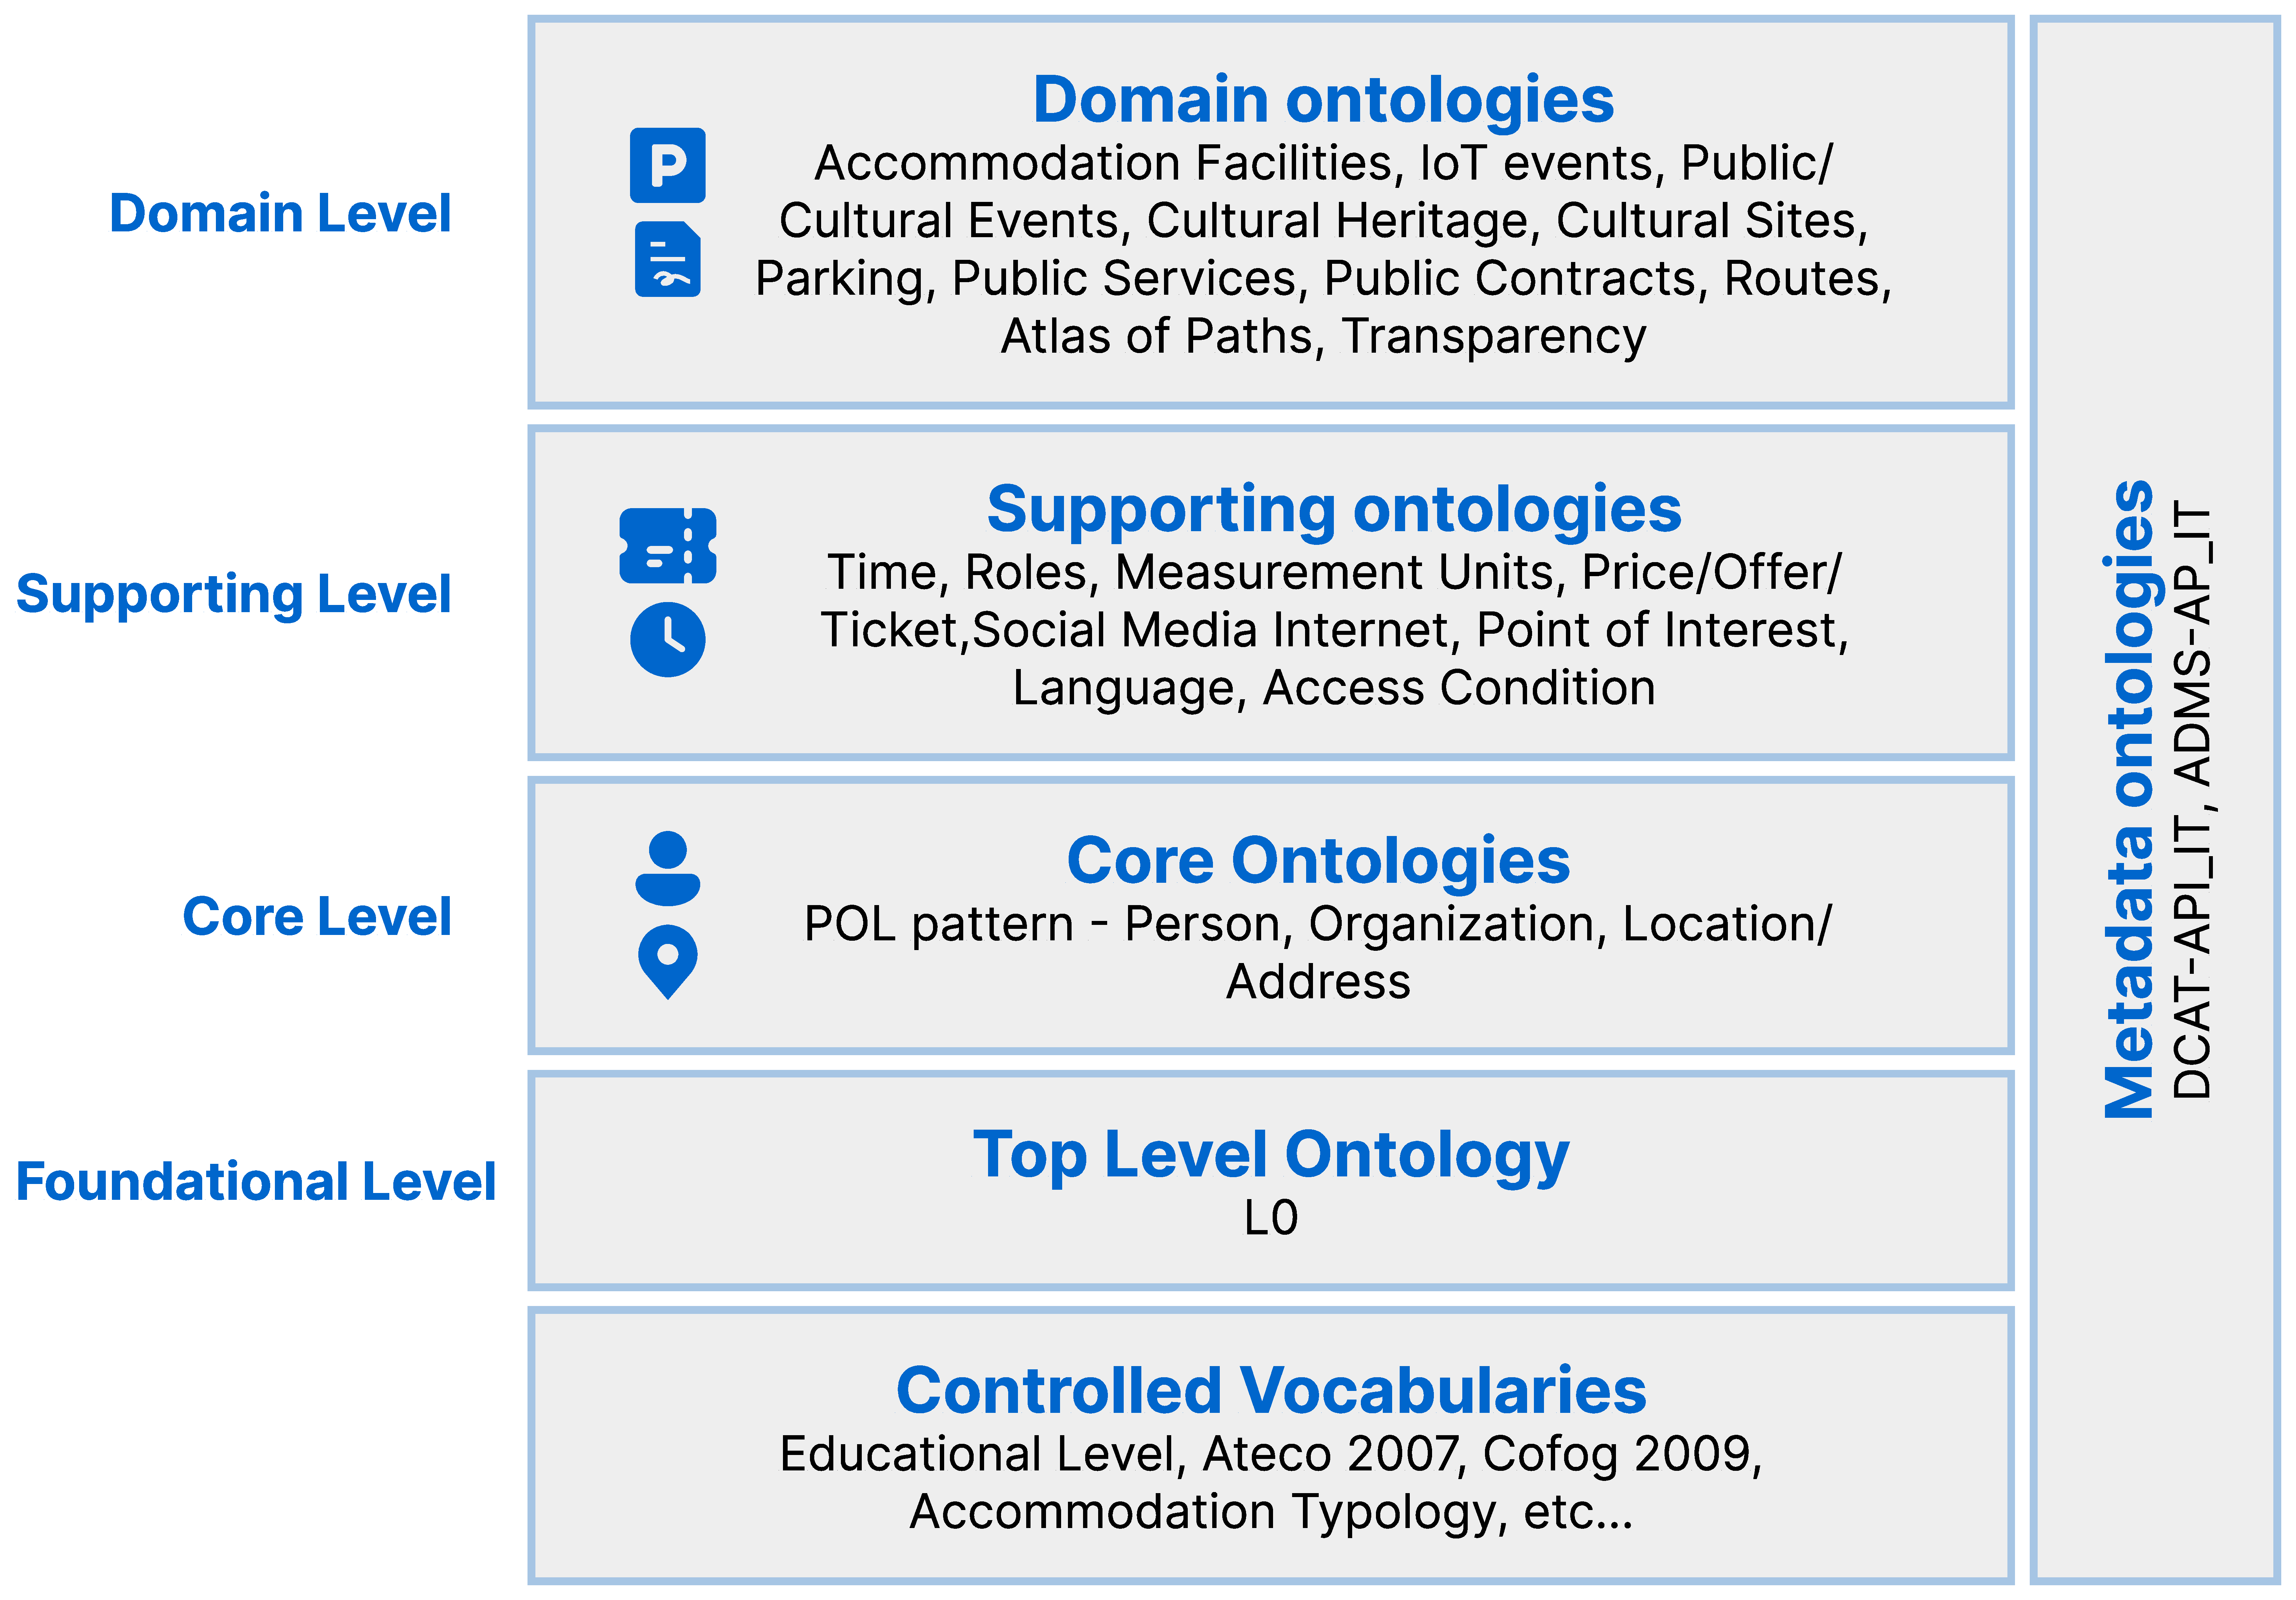
\includegraphics[width=0.8\columnwidth]{images/ontopia/ontopia-stack}
  \caption{The OntoPiA ontological stack.}
  \label{fig:ontopia-stack}
\end{figure}

\begin{longtable}[c]{lll}
  \hline
  \multicolumn{1}{|c|}{\textbf{Prefix}} & \multicolumn{1}{c|}{\textbf{\ac{URI}}}                                  & \multicolumn{1}{c|}{\textbf{Name}}         \\ \hline
  \endhead
  %
  \multicolumn{3}{|c|}{\textbf{Foundation Level}}                                                                                                                            \\ \hline
  \multicolumn{1}{|p{0.2\textwidth}|}{l0}            & \multicolumn{1}{p{0.4\textwidth}|}{\url{https://w3id.org/italia/onto/l0}}               & \multicolumn{1}{p{0.4\textwidth}|}{Level-0}                                    \\ \hline
  \multicolumn{3}{|c|}{\textbf{Core Level}}                                                                                                                                  \\ \hline
  \multicolumn{1}{|p{0.2\textwidth}|}{clvapit}       & \multicolumn{1}{p{0.4\textwidth}|}{\url{https://w3id.org/italia/onto/CLV}}              & \multicolumn{1}{p{0.4\textwidth}|}{Address (Location)}                         \\ \hline
  \multicolumn{1}{|p{0.2\textwidth}|}{covapit}       & \multicolumn{1}{p{0.4\textwidth}|}{\url{https://w3id.org/italia/onto/COV}}              & \multicolumn{1}{p{0.4\textwidth}|}{Organization (Public or Private)}           \\ \hline
  \multicolumn{1}{|p{0.2\textwidth}|}{cpvapit}       & \multicolumn{1}{p{0.4\textwidth}|}{\url{https://w3id.org/italia/onto/CPV}}              & \multicolumn{1}{p{0.4\textwidth}|}{Person}                                     \\ \hline
  \multicolumn{3}{|c|}{\textbf{Supporting Level}}                                                                                                                            \\ \hline
  \multicolumn{1}{|p{0.2\textwidth}|}{acapit}        & \multicolumn{1}{p{0.4\textwidth}|}{\url{https://w3id.org/italia/onto/AccessCondition}}  & \multicolumn{1}{p{0.4\textwidth}|}{Access Conditions}                          \\ \hline
  \multicolumn{1}{|p{0.2\textwidth}|}{langapit}      & \multicolumn{1}{p{0.4\textwidth}|}{\url{https://w3id.org/italia/onto/Language}}         & \multicolumn{1}{p{0.4\textwidth}|}{Language}                                   \\ \hline
  \multicolumn{1}{|p{0.2\textwidth}|}{muapit}        & \multicolumn{1}{p{0.4\textwidth}|}{\url{https://w3id.org/italia/onto/MU}}               & \multicolumn{1}{p{0.4\textwidth}|}{Value and Measurement Unit}                 \\ \hline
  \multicolumn{1}{|p{0.2\textwidth}|}{poiapit}       & \multicolumn{1}{p{0.4\textwidth}|}{\url{https://w3id.org/italia/onto/POI}}              & \multicolumn{1}{p{0.4\textwidth}|}{Points of Interest}                         \\ \hline
  \multicolumn{1}{|p{0.2\textwidth}|}{potapit}       & \multicolumn{1}{p{0.4\textwidth}|}{\url{https://w3id.org/italia/onto/POT}}              & \multicolumn{1}{p{0.4\textwidth}|}{Price/Offer/Ticket}                         \\ \hline
  \multicolumn{1}{|p{0.2\textwidth}|}{roapit}        & \multicolumn{1}{p{0.4\textwidth}|}{\url{https://w3id.org/italia/onto/RO}}               & \multicolumn{1}{p{0.4\textwidth}|}{Role}                                       \\ \hline
  \multicolumn{1}{|p{0.2\textwidth}|}{smapit}        & \multicolumn{1}{p{0.4\textwidth}|}{\url{https://w3id.org/italia/onto/SM}}               & \multicolumn{1}{p{0.4\textwidth}|}{Social Media/Contact and Internet}          \\ \hline
  \multicolumn{1}{|p{0.2\textwidth}|}{tiapit}        & \multicolumn{1}{p{0.4\textwidth}|}{\url{https://w3id.org/italia/onto/TI}}               & \multicolumn{1}{p{0.4\textwidth}|}{Time}                                       \\ \hline
  \multicolumn{3}{|c|}{\textbf{Domain Level}}                                                                                                                                \\ \hline
  \multicolumn{1}{|p{0.2\textwidth}|}{accoapit}      & \multicolumn{1}{p{0.4\textwidth}|}{\url{https://w3id.org/italia/onto/ACCO}}             & \multicolumn{1}{p{0.4\textwidth}|}{Accommodation Facilities}                   \\ \hline
  \multicolumn{1}{|p{0.2\textwidth}|}{aopapit}       & \multicolumn{1}{p{0.4\textwidth}|}{\url{https://w3id.org/italia/onto/AtlasOfPaths}}     & \multicolumn{1}{p{0.4\textwidth}|}{Atlas of Paths}                             \\ \hline
  \multicolumn{1}{|p{0.2\textwidth}|}{chapit}        & \multicolumn{1}{p{0.4\textwidth}|}{\url{https://w3id.org/italia/onto/CulturalHeritage}} & \multicolumn{1}{p{0.4\textwidth}|}{Cultural Heritage}                          \\ \hline
  \multicolumn{1}{|p{0.2\textwidth}|}{cis}           & \multicolumn{1}{p{0.4\textwidth}|}{\url{http://dati.beniculturali.it/cis}}              & \multicolumn{1}{p{0.4\textwidth}|}{Cultural Institute/Site and Cultural Event} \\ \hline
  \multicolumn{1}{|p{0.2\textwidth}|}{cpevapit}      & \multicolumn{1}{p{0.4\textwidth}|}{\url{https://w3id.org/italia/onto/CPEV}}             & \multicolumn{1}{p{0.4\textwidth}|}{Public Events}                              \\ \hline
  \multicolumn{1}{|p{0.2\textwidth}|}{cpsvapit}      & \multicolumn{1}{p{0.4\textwidth}|}{\url{https://w3id.org/italia/onto/CPSV}}             & \multicolumn{1}{p{0.4\textwidth}|}{Public Services}                            \\ \hline
  \multicolumn{1}{|p{0.2\textwidth}|}{herapit}       & \multicolumn{1}{p{0.4\textwidth}|}{\url{https://w3id.org/italia/onto/HER}}              & \multicolumn{1}{p{0.4\textwidth}|}{Higher Education and Research}              \\ \hline
  \multicolumn{1}{|p{0.2\textwidth}|}{indicator}     & \multicolumn{1}{p{0.4\textwidth}|}{\url{https://w3id.org/italia/onto/Indicator}}        & \multicolumn{1}{p{0.4\textwidth}|}{Indicator}                                  \\ \hline
  \multicolumn{1}{|p{0.2\textwidth}|}{iotapit}       & \multicolumn{1}{p{0.4\textwidth}|}{\url{https://w3id.org/italia/onto/IoT}}              & \multicolumn{1}{p{0.4\textwidth}|}{IoT event}                                  \\ \hline
  \multicolumn{1}{|p{0.2\textwidth}|}{parkapit}      & \multicolumn{1}{p{0.4\textwidth}|}{\url{https://w3id.org/italia/onto/PARK}}             & \multicolumn{1}{p{0.4\textwidth}|}{Parking}                                    \\ \hline
  \multicolumn{1}{|p{0.2\textwidth}|}{pcapit}        & \multicolumn{1}{p{0.4\textwidth}|}{\url{https://w3id.org/italia/onto/PublicContract}}   & \multicolumn{1}{p{0.4\textwidth}|}{Public Contracts}                           \\ \hline
  \multicolumn{1}{|p{0.2\textwidth}|}{prjapit}       & \multicolumn{1}{p{0.4\textwidth}|}{\url{https://w3id.org/italia/onto/Project}}          & \multicolumn{1}{p{0.4\textwidth}|}{Project}                                    \\ \hline
  \multicolumn{1}{|p{0.2\textwidth}|}{rtapit}        & \multicolumn{1}{p{0.4\textwidth}|}{\url{https://w3id.org/italia/onto/Route}}            & \multicolumn{1}{p{0.4\textwidth}|}{Routes}                                     \\ \hline
  \multicolumn{1}{|p{0.2\textwidth}|}{trapit}        & \multicolumn{1}{p{0.4\textwidth}|}{\url{https://w3id.org/italia/onto/Transparency}}     & \multicolumn{1}{p{0.4\textwidth}|}{Transparency Obligations}                   \\ \hline
  \multicolumn{3}{|c|}{\textbf{Metadata}}                                                                                                                                    \\ \hline
  \multicolumn{1}{|p{0.2\textwidth}|}{admsapit}      & \multicolumn{1}{p{0.4\textwidth}|}{\url{https://w3id.org/italia/onto/ADMS}}             & \multicolumn{1}{p{0.4\textwidth}|}{Asset Description Metadata Schema}          \\ \hline
  \multicolumn{1}{|p{0.2\textwidth}|}{dcatapit}      & \multicolumn{1}{p{0.4\textwidth}|}{\url{https://w3id.org/italia/onto/DCAT}}             & \multicolumn{1}{p{0.4\textwidth}|}{Data Catalog Vocabulary}                   \\ \hline
  \caption{Ontologies part of the OntoPiA network.}
  \label{tab:ontopia-ontologies}\\
\end{longtable}